\documentclass[10pt,mathserif]{beamer}

\usepackage{graphicx,amsmath,amssymb,tikz,psfrag,subfigure,bm}

\input defs.tex

%% formatting

\mode<presentation>
{
\usetheme{default}
}
\setbeamertemplate{navigation symbols}{}
\usecolortheme[rgb={0,0,0}]{structure}
\setbeamertemplate{itemize subitem}{--}
\setbeamertemplate{frametitle} {
	\begin{center}
	  {\large\bf \insertframetitle}
	\end{center}
}

\AtBeginSection[] 
{ 
	\begin{frame}<beamer> 
		\frametitle{Outline} 
		\tableofcontents[currentsection,currentsubsection] 
	\end{frame} 
} 

%% begin presentation

\title{\large \bfseries Kernels}

\author{Jiali Lin\\[3ex]
Virginia Tech}

\date{\today}

\begin{document}

\frame{
\thispagestyle{empty}
\titlepage
}

\section{Kernel functions}
\begin{frame}{Introduction}
\begin{itemize}
    \item \textbf{Goal:} measure the similarity between objects, that doesn't require preprocessing them into feature vector format.
    \item E.g. when comparing strings, we can compute the edit distance between them.
    \item \textbf{Kernel function} $\kappa (\bm{x}, \bm{x'})$: some measure of similarity between objects $\bm{x}, \bm{x'}\in\mathcal{\bm{X}}$ , where $\mathcal{\bm{X}}$ is some abstract space.
\end{itemize}
\end{frame}

\begin{frame}{Mercer Kernel Functions}
\begin{itemize}
    \item A kernel function maps pairs of inputs to real numbers
    \begin{equation*}
        \kappa: \mathcal{\bm{X}} \times \mathcal{\bm{X}} \rightarrow \mathbb{R} \quad\quad \kappa (\bm{x}_i, \bm{x}_j) = \kappa(\bm{x}_j, \bm{x}_i)
    \end{equation*}
    Intuition: Larger values indicate inputs are``more similar".
    \item A kernel function is positive semidefinite if and only if for any $n\geq1$, and any $x = \{\bm{x}_1, \bm{x}_2,\ldots,\bm{x}_n\}$, the Gram matrix is positive semidefinite
    \begin{equation*}
        \bm{K} \in \mathbb{R}^{n \times n}\quad\quad K_{ij} = \kappa (\bm{x}_i, \bm{x}_j)
    \end{equation*}
    \item \textbf{Mercer's Theorem}: Assuming certain technical conditions, every positive definite kernel function can be represented as
    \begin{equation*}
        \kappa (\bm{x}_i, \bm{x}_j) = \sum_{\ell=1}^d\phi_\ell(\bm{x}_i)\phi_\ell(\bm{x}_j)
    \end{equation*}
    \item \textbf{Motivation}: Can be faster to compute kernel than features.
\end{itemize}
\end{frame}

\begin{frame}{RBF kernels}
\begin{itemize}
    \item The \textbf{squared exponential kernel} (SE kernel) or \textbf{Gaussian kernel}
    \begin{equation*}
        \kappa (\bm{x}, \bm{x'}) = \exp(-\frac{1}{2}(\bm{x}-\bm{x'})^T \bm{\Sigma}^{-1} (\bm{x}-\bm{x'}))
    \end{equation*}
    \item If $\bm{\Sigma}^{-1}$ is diagonal, this can be written as
    \begin{equation*}
        \kappa(\bm{x}, \bm{x'}) = \exp(-\frac{1}{2} \sum_{j=1}^D \frac{1}{\sigma^2_j }(\bm{x}_j - \bm{x}_j')^2)
    \end{equation*}
    \item We can interpret the $\sigma_j$ as defining the \textbf{characteristic length scale} of dimension $j$. 
    \item \textbf{ARD kernel}: If $\sigma_j = \infty$, the corresponding dimension is ignored.
    \item \textbf{Radial basis function:} If $\bm{\Sigma}$ is spherical, we get the isotropic kernel
    \begin{equation*}
        \kappa(\bm{x}, \bm{x'}) = \exp(-\frac{\|\bm{x}-\bm{x'}\|^2}{2\sigma^2} )
    \end{equation*}
    $\sigma^2$ is \textbf{bandwidth}. \textbf{RBF} kernel is only a function of $\|\bm{x}-\bm{x'}\|$.
\end{itemize}
\end{frame}

    
\begin{frame}{Polynomial Kernels}
\begin{itemize}
    \item $\mathcal{\bm{X}} \rightarrow$ real vectors of some fixed dimension. 
    \item \textbf{Polynomial kernel} 
    \begin{equation*}
        \kappa (\bm{x}, \bm{x'}) = (\gamma \bm{x}^T \bm{x}' + r)^M, \quad\text{where}\quad r > 0
    \end{equation*}
    \item If $M = 2, \gamma = r = 1$ and $x, x' \in \mathbb{R}^2$, we have
    \begin{equation*}
        \begin{split}
            (1 + \bm{x}^T \bm{x'})^2 & = (1 + \bm{x}_1\bm{x}_1' + \bm{x}_2\bm{x}_2')^2\\
            & = 1 + 2\bm{x}_1\bm{x}_1' + 2\bm{x}_2\bm{x}_2' + (\bm{x}_1\bm{x}_1')^2 + (\bm{x}_2\bm{x}_2')^2 + 2\bm{x}_1\bm{x}_1'\bm{x}_2\bm{x}_2'\\
            & = \bm{\phi}(\bm{x})^T \bm{\phi}(\bm{x})
        \end{split}
    \end{equation*}
    where $\bm{\phi}(\bm{x}) = [1, \sqrt{2} \bm{x}_1, \sqrt{2} \bm{x}_2, \bm{x}_1^2, \bm{x}_2^2, \sqrt{2} \bm{x}_1\bm{x}_2]^T$
    \item This is equivalent to working in a 6 dimensional feature space. 
    \item In the case of a Gaussian kernel, the feature map lives in an infinite dimensional space. 
\end{itemize}
\end{frame}

\begin{frame}{Linear kernels}
\begin{itemize}
    \item Deriving the feature vector implied by a kernel is in general quite difficult, and only possible if the kernel is Mercer.
    \item However, deriving a kernel from a feature vector is easy: we just use
    \begin{equation*}
        \kappa (\bm{x}, \bm{x'}) = \bm{\phi}(\bm{x})^T \bm{\phi}(\bm{x}) = <\bm{\phi}(\bm{x}), \bm{\phi}(\bm{x}')>
    \end{equation*}
    \item If $\bm{\phi}(\bm{x}) = \bm{x}$, we get the linear kernel, defined by
    \begin{equation*}
        \kappa (\bm{x}, \bm{x'}) = \bm{x}^T \bm{x'}
    \end{equation*}
\end{itemize}
\end{frame}

\section{The kernel trick}
\begin{frame}{Kernelized ridge regression}
The primal problem:
\begin{itemize}
    \item Let $\bm{x} \in \mathbb{R}^D$ be some feature vector, and $\bm{X}$ be the corresponding $N \times D$ design matrix. We want to minimize
    \begin{equation*}
        J(\bm{w}) = (\bm{y} - \bm{X}\bm{w})^T (\bm{y} - \bm{X}\bm{w}) + \lambda\|\bm{w}\|^2
    \end{equation*} 
    \item The optimal solution is given by
    \begin{equation*}
        \bm{w} = (\bm{X}^T \bm{X}+\lambda \bm{I}_D)^{-1} \bm{X}^T \bm{y} =(\sum_i \bm{\bm{x}_i\bm{x}_i^T} +\lambda \bm{I}_D)^{-1}\bm{X}^T \bm{y}
    \end{equation*}
\end{itemize}
\end{frame}
        
\begin{frame}{Kernelized ridge regressionc(cont'd)}
The dual problem:
\begin{itemize}
    \item Rewrite the ridge estimate by the matrix inversion lemma
    \begin{equation*}
        \bm{w} = \bm{X}^T(\bm{X}\bm{X}^T +\lambda \bm{I}_N)^{-1}\bm{y} 
    \end{equation*}
    \item Why?
    \begin{itemize}
        \item This can be computationally advantageous if $D$ is large.
        \item Partially kernelize this, by replacing $\bm{X}\bm{X}^T$ with the Gram matrix $\bm{K}$.
    \end{itemize}
    \item What about the leading $\bm{X}^T$ term?
    \begin{itemize}
        \item Define the following \textbf{dual variables}
        \begin{equation*}
            \alpha =  (\bm{K} + \lambda \bm{I}_N)^{-1}\bm{y}
        \end{equation*}
        \item  Then we can rewrite the primal variables as follows
    \begin{equation*}
        \bm{w} = \bm{X}^T\alpha = \sum_{i=1}^N \alpha_i \bm{\bm{x}_i}
    \end{equation*}
    \item  Plug this in at test time to compute the predictive mean, we get
        \begin{equation*}
            \hat{f}(\bm{x}) = \bm{w^T x} = \sum_{i=1}^N \alpha_i \bm{\bm{x}_i^T x} = \sum_{i=1}^N \alpha_i\kappa(\bm{x,\bm{x}_i})
        \end{equation*}
    \end{itemize}
\end{itemize}
\end{frame}

\section{Support vector machines}
\begin{frame}{Introduction}
\begin{itemize}
    \item Consider the $\ell_2$ regularized empirical risk function
    \begin{equation*}
        J(\bm{w}, \lambda) = \sum_{i=1}^NL(y_i, \hat{y}_i) + \lambda\|\bm{w}\|^2
    \end{equation*}
    \item \textbf{Support vector machine}: use a modified loss function to ensure that the solution is sparse, so that predictions only depend on a subset of the training data.
    \item SVMs are very unnatural from a probabilistic point of view.
    \begin{itemize}
        \item SVMs encode sparsity in the loss function rather than the prior.
        \item SVMs encode kernels by using an algorithmic trick, rather than being an explicit part of the model.
        \item SVMs do not result in probabilistic outputs (nonparametric).
    \end{itemize}
\end{itemize}
\end{frame}

\begin{frame}{Losses for Binary Classification}
\begin{equation*}
    \hat{\bm{w}} = \argmin_{\bm{w}} \frac{\lambda}{2}\|\bm{w}\|^2 + \sum_{i=1}^n L(\tilde{y_i} \bm{w}^T\phi(\bm{x}_i)), \quad \text{where} \quad \tilde{y_i}\in\{+1, -1\}
\end{equation*}
\begin{figure}[h]
\centering
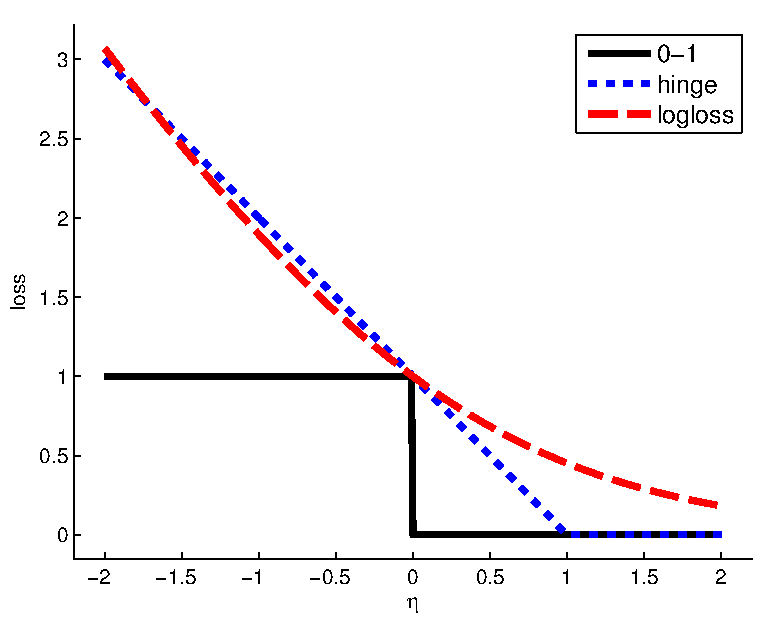
\includegraphics[width=0.5\textwidth]{hingeLoss}
\caption{Illustration of various loss functions for binary classification. The horizontal axis is the margin $y\eta$, the vertical axis is the loss. The log loss uses log base 2. Figure generated by \texttt{HingeLossPlot}.}
\end{figure}
\end{frame}

\begin{frame}{Losses for Binary Classification (cont'd)}
\begin{itemize}
\item Training Error Rate (0-1 loss) 
\begin{itemize}
    \item For many classifications, the objective we really care about.
    \item \textcolor{red}{Hard to optimize (gradients zero almost everywhere)}.
    \item \textcolor{red}{Cannot distinguish top-performing training classifiers}.
\end{itemize}

\item  Logistic Regression (logarithmic loss)
\begin{itemize}
    \item \textcolor{blue}{Estimates label probabilities for calibrated decision-making}.
    \item \textcolor{blue}{Easy to optimize (convex, smooth bound on 0-1 loss)}.
    \item \textcolor{red}{Scalability problems with large datasets and many features}.
\end{itemize}

\item Support Vector Machine (hinge loss)
\begin{itemize}
    \item \textcolor{red}{Does not estimate valid probability distribution on labels}.
    \item Possible to optimize (convex, non-smooth bound on $0-1$ loss).
    \item \textcolor{blue}{Chooses boundary which maximizes margin of training data}.
    \item \textcolor{blue}{Gives sparse solutions, allowing greater scalability}.
\end{itemize}    
\end{itemize}
\end{frame}

\begin{frame}{Support Vector Machines (SVMs) }
\begin{itemize}
    \item \textbf{Goal}
    \begin{equation*}
    \hat{\bm{w}} = \argmin_{\bm{w}} \frac{\lambda}{2}\|\bm{w}\|^2 + \sum_{i=1}^n L(\tilde{y_i} \bm{w}^T\phi(\bm{x}_i))
    \end{equation*}
    \item \textbf{Hinge loss}
    \begin{equation*}
        L_{\text{hinge}}(y, \eta) = \max(0, 1 - y\eta) = (1 - y\eta)_+
    \end{equation*}
    \item \textbf{SVM Penalized Objective}
    \begin{equation*}
    \hat{\bm{w}} = \argmin_{\bm{w}} \frac{\lambda}{2}\|\bm{w}\|^2 + \sum_{i=1}^n (1-\tilde{y_i} \bm{w}^T\phi(\bm{x}_i))_+
    \end{equation*}
    \item \textbf{SVM Constrained Objective}
    \begin{equation*}
        \begin{split}
            & \argmin_{\bm{w},\xi} \frac{1}{2}\|\bm{w}\|^2 + C\sum_{i=1}^N (\xi_i)\\
            \text{s.t.} & \quad \xi_i\geq 0, \quad \tilde{y_i} \bm{w}^T\phi(\bm{x}_i)\geq 1-\xi_i
        \end{split}
    \end{equation*}
    \begin{itemize}
    \item Quadratic Program: Quadratic function with linear constraints.
    \item \textbf{Slack Variables}: $\bm{x}_i$ penalize misclassified training examples.
    \end{itemize}
\end{itemize}
\end{frame}

\begin{frame}{Maximum Margin Hyperplanes}
\begin{figure}[h]
\centering
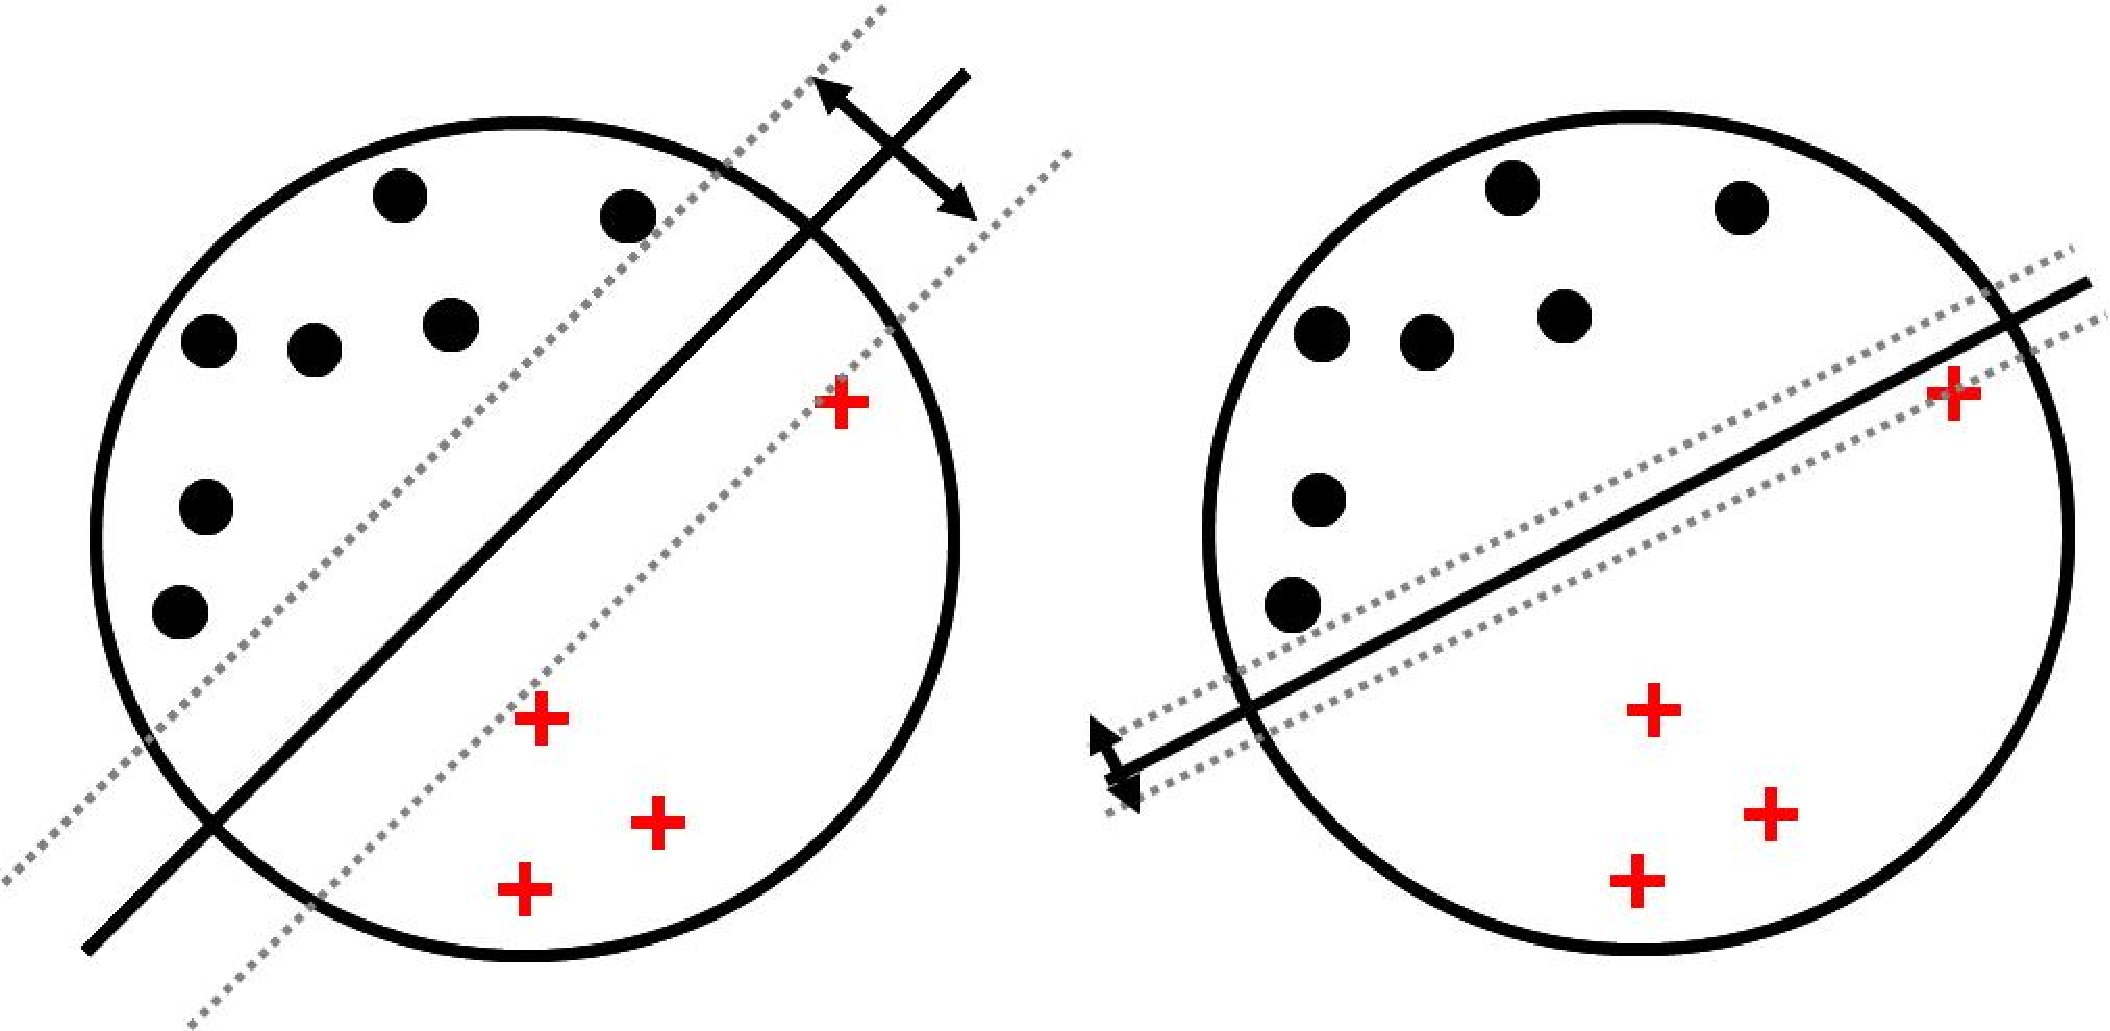
\includegraphics[width=0.5\textwidth]{largeMarginPrinciple2}
\caption{Illustration of the large margin principle. Left: a separating hyper-plane with large margin. Right: a separating hyper-plane with small margin.}
\end{figure}
\begin{itemize}
    \item \textbf{Margin}: For a hyperplane which perfectly separates training data, orthogonal distance of closest training example to plane.
    \item \textbf{Intuition}: Expect similar features to have similar labels, so would like decision boundary as far as possible from data.
    \item Statistical Learning Theory: Formal bounds on generalization performance (test error) of large-margin classifiers.
    \end{itemize}
\end{frame}

\begin{frame}{Maximum Margin Hyperplanes (cont'd)}
\begin{figure}[h]
\centering     %%% not \center
\subfigure[]{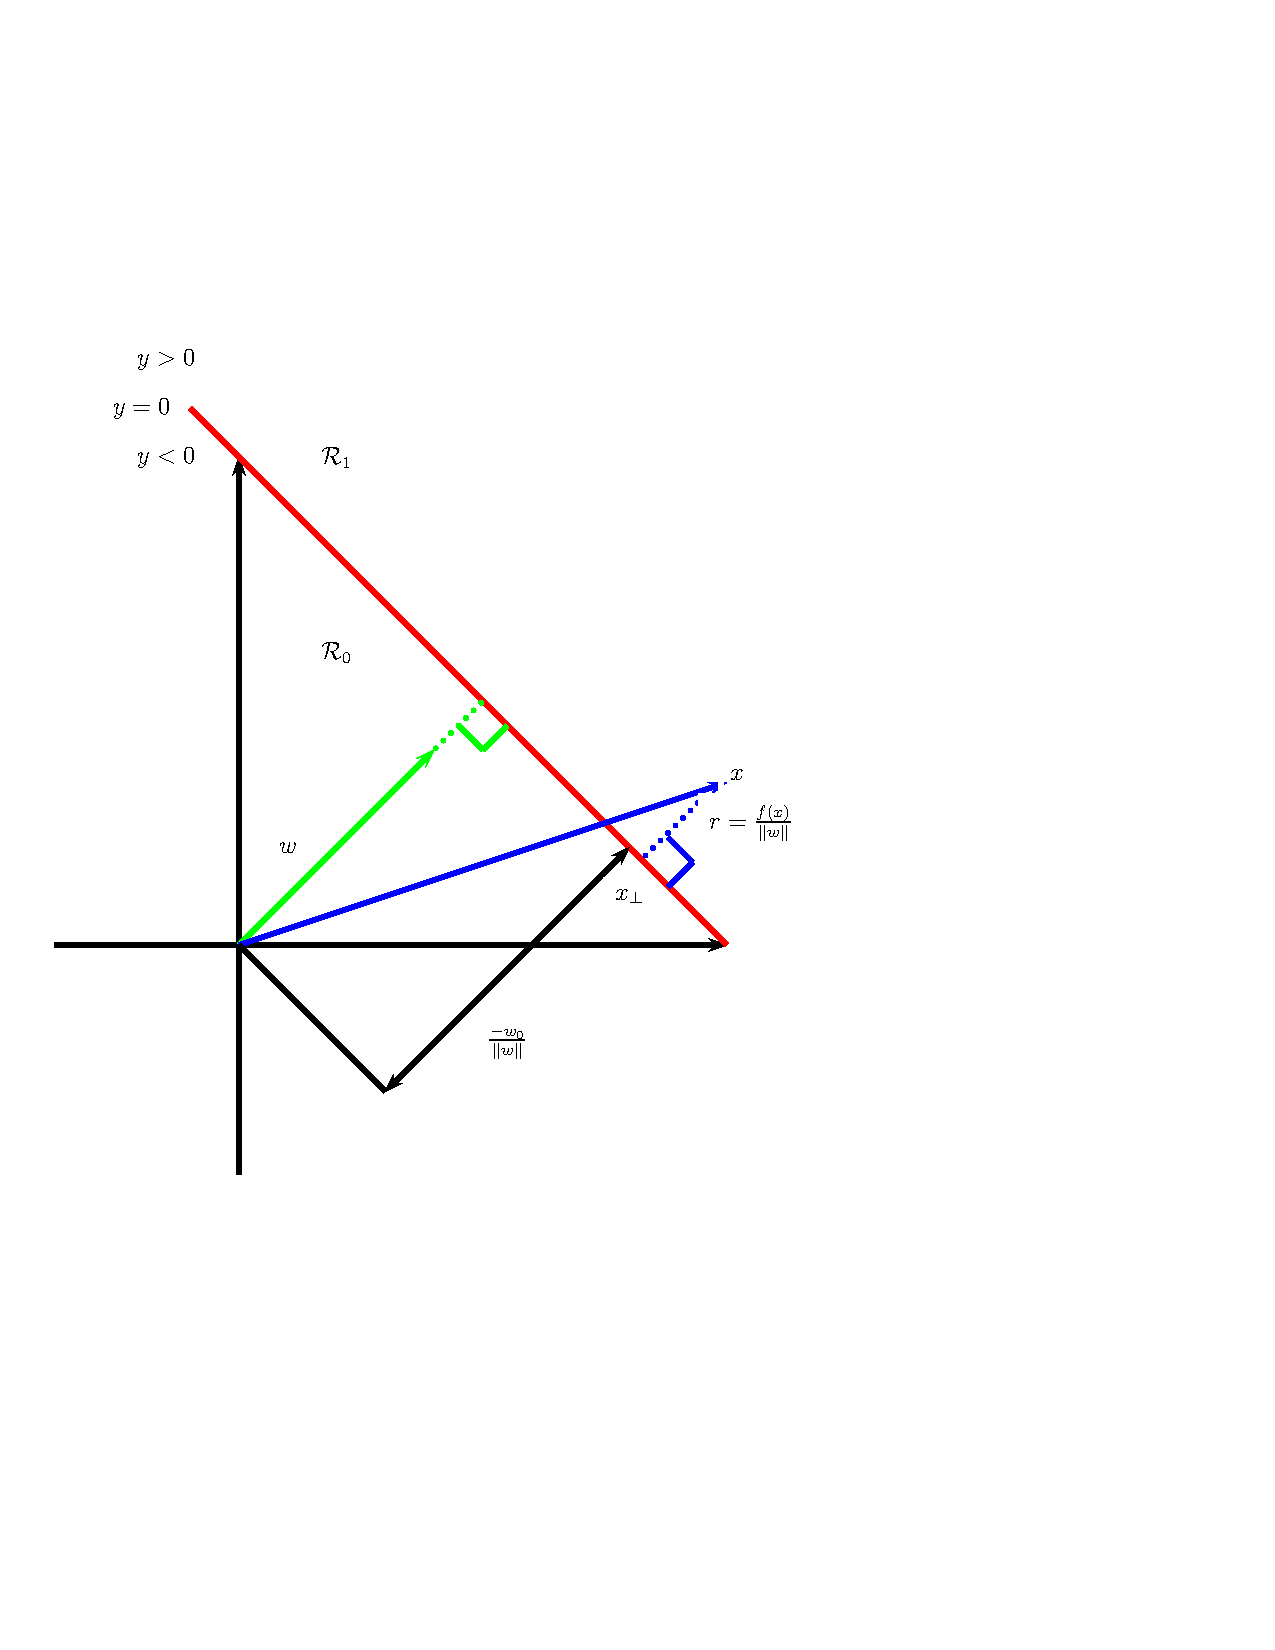
\includegraphics[width=40mm]{geomLinDiscrim}}
\subfigure[]{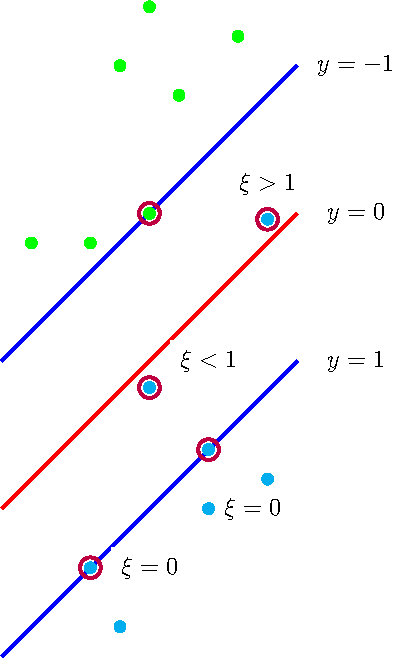
\includegraphics[width=30mm]{softMargin}}
\caption{(a) Geometry of a linear decision boundary. (b) Soft margin principle.}
\end{figure}
\end{frame}

\begin{frame}{Maximum Margin Hyperplanes (cont'd)}
\begin{itemize}
    \item Referring to Figure, $\bm{w}$ is perpendicular to the boundary, so $\overrightarrow{\bm{x}_\perp \bm{x}}$ is parallel to $\bm{w}$, i.e. $\overrightarrow{\bm{x}_\perp \bm{x}}  = r\frac{\bm{w}}{\|\bm{w}\|}$.
    \item Thus, $\bm{x} = \bm{x}_\perp + r\frac{\bm{w}}{\|\bm{w}\|}$,
    where $r$ is the distance of $\bm{x}$ from the decision boundary whose normal vector is $\bm{w}$, and $\bm{x}_\perp$ is the orthogonal projection of $\bm{x}$ onto this boundary. 
    \item Multiply both sides by $\bm{w}^T$ and plus $w_0$ to get $f(\bm{x}) = f(\bm{\bm{x}}_\perp)+r\|\bm{w}\|$. Now $f(\bm{x}_\perp) = 0$, thus $r = \frac{f(\bm{x})}{\|\bm{w}\|}$.
\end{itemize}
\end{frame}

\begin{frame}{Margins and SVMs}
\begin{itemize}
    \item Let $\phi(\bm{x}) = \bm{x}_\perp + r\frac{\bm{w}}{\|\bm{w}\|}$.
    \item Now make this distance $r = \frac{f(\bm{x})}{\|\bm{w}\|}$ as large as possible. 
    \item Accuracy: Classify all training data correctly by enforcing
    \begin{equation*}
        \tilde{y_i} \bm{w}^T\phi(\bm{x}_i) > 0
    \end{equation*}
    \item Margin: Maximize distance of closest point to boundary 
    \begin{equation*}
        \max_{w_0,\bm{w}}\min_{i=1,\ldots n}\frac{\tilde{y_i} \bm{w}^T\phi(\bm{x}_i)}{\|\bm{w}\|}
    \end{equation*}
    \item Invariance: Scale $\bm{w}$ so closest point distance 1 from boundary 
    \begin{equation*}
        \begin{split}
            & \argmin_{\bm{w},\xi} \frac{1}{2}\|\bm{w}\|^2 + C\sum_{i=1}^N (\xi_i)\\
            \text{s.t.} & \quad \xi_i\geq 0, \quad \tilde{y_i} \bm{w}^T\phi(\bm{x}_i)\geq 1-\xi_i
        \end{split}
    \end{equation*}
\end{itemize}
\end{frame}

\begin{frame}{Support Vectors and Sparsity}
\begin{equation*}
    \hat{\bm{w}} = \argmin_{\bm{w}} \frac{\lambda}{2}\|\bm{w}\|^2 + \sum_{i=1}^n (1-\tilde{y_i} \bm{w}^T\phi(\bm{x}_i))_+
\end{equation*}
\begin{itemize}
    \item Optimal solution takes following form:
    \begin{equation*}
        \hat{\bm{w}} = \sum_{i=1}^n \alpha_i \tilde{y_i} \bm{w}^T\phi(\bm{x}_i)\quad\alpha_i>0
    \end{equation*}
    \item Here, the $\alpha_i$ are Lagrange multipliers for constrained QP.
    \item Because loss exactly zero for arguments greater than one, only a sparse subset of training examples have $\alpha_i>0$.
    \item Training examples with non-zero weight are support vectors.
    \item \textbf{Optimization}: quadratic program solver.
    \item Improvement: \textbf{sequential minimal optimization} or \textbf{SMO} algorithm.
\end{itemize}
\end{frame}

\begin{frame}{SVMs and Kernels}
\begin{itemize}
    \item Optimal weights always the form, with non-zero weights only for support vectors
    \begin{equation*}
        \bm{w} = \sum_{j=1}^n \beta_j \phi(\bm{x}_j)
    \end{equation*}
    \item Kernel Tricks: for $\bm{K} \in \mathbb{R}^{n \times n}$, $K_{ij} = \kappa(\bm{x}_i,\bm{x}_j) = \phi(\bm{x}_i)^T \phi(\bm{x}_j)$.
    \item Then $\bm{f} = \bm{K}\bm{\beta}$,  $f_i = \bm{w}^T\phi(\bm{x}_i)$. Thus, $\|\bm{w}\|^2 = \bm{f}^T\bm{K}^{-1}\bm{f}$.
    \item Dual SVM
    \begin{equation*}
        \hat{\bm{f}} = \argmin_{\bm{f}} \frac{\lambda}{2}\bm{f}^T \bm{K}^{-1}\bm{f} + \sum_{i=1}^n (1-\tilde{y_i} \bm{w}^T\phi(\bm{x}_i))_+
    \end{equation*}
    \item Primal SVM
    \begin{equation*}
        \hat{\bm{w}} = \argmin_{\bm{w}} \frac{\lambda}{2}\|\bm{w}\|^2 + \sum_{i=1}^n (1-\tilde{y_i} \bm{w}^T\phi(\bm{x}_i))_+
    \end{equation*}
\end{itemize}
\end{frame}

\begin{frame}{SVMs and Gaussian Processes}
\begin{itemize}
    \item Logistic Regression
    \begin{equation*}
        \hat{\bm{w}} = \argmin_{\bm{w}} \frac{\lambda}{2}\|\bm{w}\|^2 + \sum_{i=1}^n \log(1+ e^{\tilde{y_i} \bm{w}^T\phi(\bm{x}_i)})
    \end{equation*}
    \item GP Classification
    \begin{equation*}
        \hat{\bm{f}} = \argmin_{\bm{f}} \frac{\lambda}{2}\bm{f}^T \bm{K}^{-1}\bm{f} + \sum_{i=1}^n \log(1+ e^{\tilde{y_i} f_i})
    \end{equation*}
    \item Dual SVM
    \begin{equation*}
        \hat{\bm{f}} = \argmin_{\bm{f}} \frac{\lambda}{2}\bm{f}^T \bm{K}^{-1}\bm{f} + \sum_{i=1}^n (1-\tilde{y_i} \bm{w}^T\phi(\bm{x}_i))_+
    \end{equation*}
    \item Primal SVM
    \begin{equation*}
        \hat{\bm{w}} = \argmin_{\bm{w}} \frac{\lambda}{2}\|\bm{w}\|^2 + \sum_{i=1}^n (1-\tilde{y_i} \bm{w}^T\phi(\bm{x}_i))_+
    \end{equation*}
\end{itemize}
\end{frame}

\end{document}

